\section{Containers}
\label{sec:background:containers}


% General introduction Container
A \gls{container} is a unit of executable software that is packaged with all of its dependencies \cite{docker-what-is-container, ibm-what-is-container}. By packaging everything in a single unit it makes it easy to run the application on different environments, from desktops and laptops to cloud environments. \Glspl{container} isolate software from their environment and ensure that it works uniformly on all devices regardless of operating systems used or the hardware powering it. 




% How it works
\Glspl{container} leverage a set of Linux technologies, such as \textit{cgroups} and \textit{namespaces}. The former is a mechanism to organize processes in hierarchical groups whose usage of various system resources can then be limited and monitored \cite{cgroups, man-cgroups}. The latter is a technology to wrap a system resource in an abstraction to make it appear to a process as if they had their own isolated instance of that resource \cite{man-namespaces}. These combined with the fact that a container has a layered file system that contains the application code and operating system dependencies makes it so that it is a fast and lightweight unit of compute. 

A comparison with \glspl{vm} is commonly made because of their isolating properties and abstractions. However, a \gls{vm} is a software-based virtualization of an entire computer system, this includes the hardware, the entire operating system that runs on it in addition to the applications and binaries that it requires. A \gls{container} on the other hand is an abstraction at the application level, where it is simply just another process living in user space. A comparison of the different deployment models can be seen in \ref{fig:vm-vs-container}.


\begin{figure}[!t]
    \centering
    
    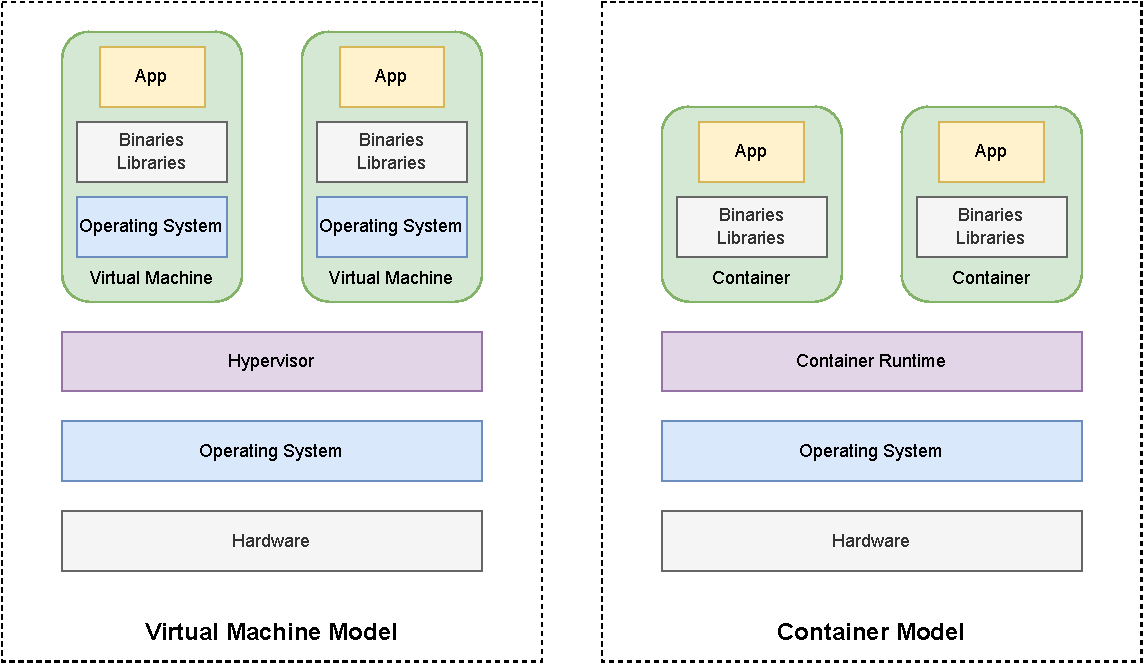
\includegraphics[width=.9\linewidth]{2_background/figures/vm-vs-container.pdf}

    \caption[Container and Virtual Machine-based deployment models]{Container and Virtual Machine-based deployment models.}
    \label{fig:vm-vs-container}
\end{figure}

% Docker 
\Gls{docker} was introduced in Santa Clara at PyCon in 2013 \cite{pycon2013}. It jump started the revolution of \glspl{container} and was for many the first introduction to \gls{container} technologies. It was loved by developers for its portability and speed compared to traditional \gls{vm} deployments that were commonly used. Due to its immense popularity and praise, which it has managed to uphold according to recent surveys as conducted by stack overflow \cite{stack-overflow-survey}, \gls{docker} became the de facto standard in \gls{container} technologies and the similarly named company decided in 2015 to establish an open-source initiative that governs \gls{container} related standards \cite{open-container-standard}. Along with this they donated their container image specification format \cite{open-container-standard-image-spec} to this initiative as an open-source contribution. With this image specification standard in place, others could develop compatible container runtimes which were able to run the container images produced by said specification.
